\section{Основные шаги вычисления}

\begin{figure}
    \centering
    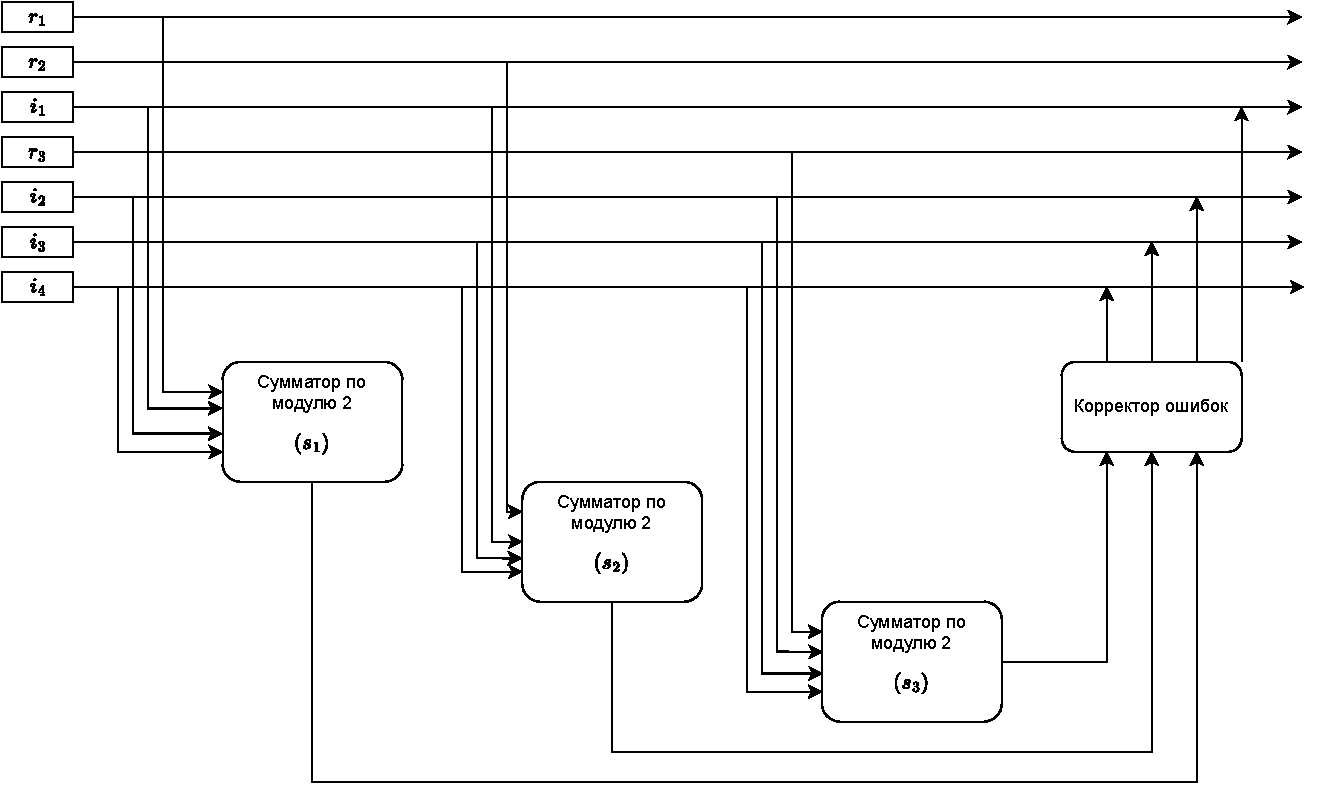
\includegraphics[scale=0.7]{img/74.pdf}
    \caption{Схема декодирования классического кода Хэмминга $(7; 4)$}
\end{figure}

\begin{figure}
    \centering
    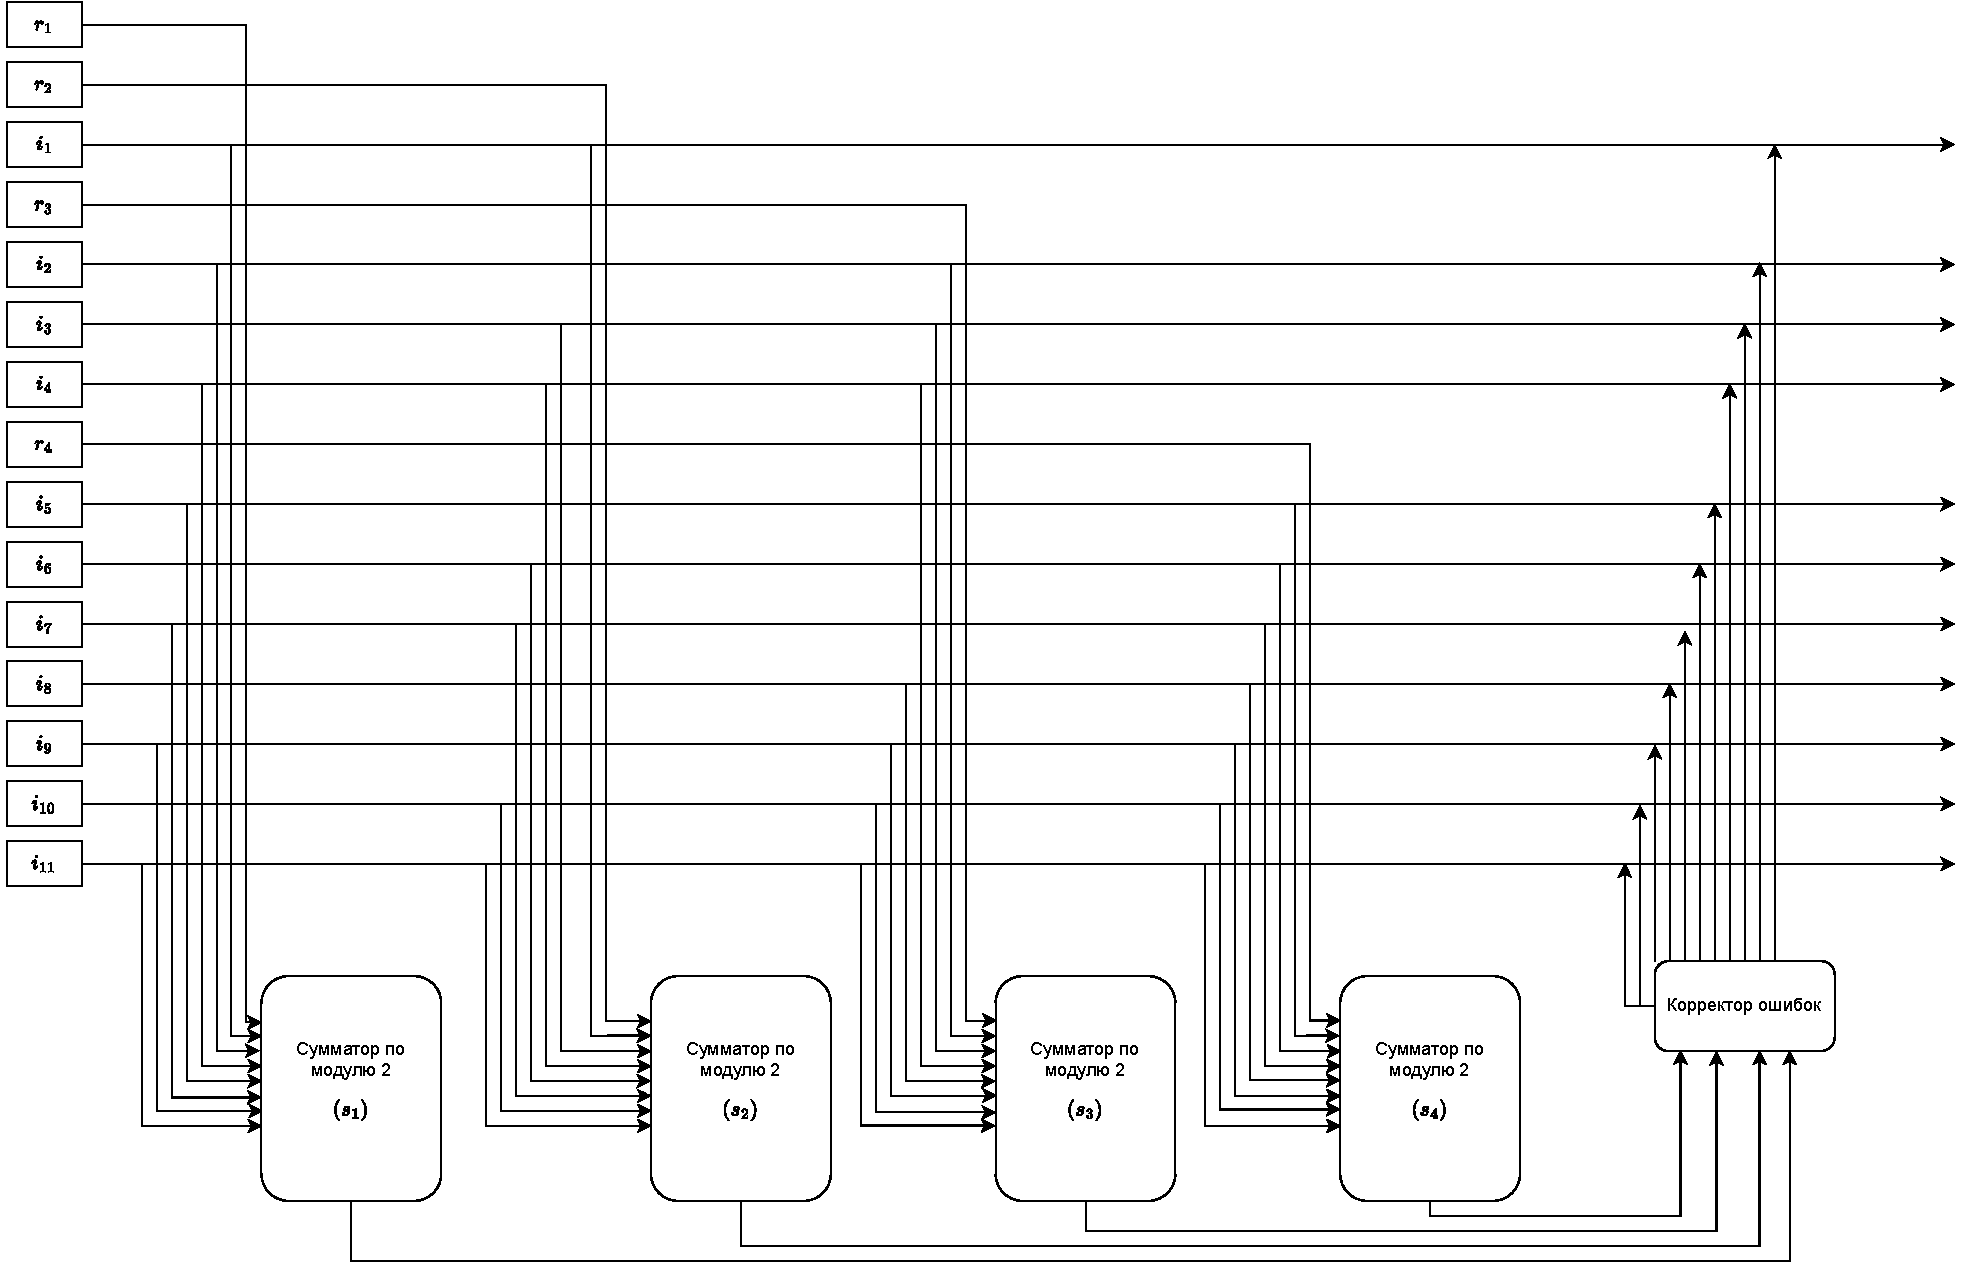
\includegraphics[scale=0.5]{img/1511.pdf}
    \caption{Схема декодирования классического кода Хэмминга $(15; 11)$}
\end{figure}


\begin{enumerate}
    \item Посчитаем $s_1, s_2, s_3$. $s_1 = r_1 \oplus i_1 \oplus i_2 \oplus i_4 = 0 \oplus 0 \oplus 1 \oplus 0 = 1$
    $s_2 = r_2 \oplus i_1 \oplus i_3 \oplus i_4 = 0 \oplus 0 \oplus 1 \oplus 0 = 1$.
    $s_3 = r_3 \oplus i_2 \oplus i_3 \oplus i_4 = 0 \oplus 1 \oplus 1 \oplus 0 = 0$.
    Запишем в обратном порядке, получаем $011$, переведем в десятичную СС, значит ошибка в 3-м бите, то есть $i_1$.
    Тогда корректное значение $i_1 := i_1 \oplus 1 = 1$.
    Получается, что итоговое сообщение: $1110$.

    \item Посчитаем $s_1, s_2, s_3$. $s_1 = 1$, $s_2 = 1$, $s_3= 0$. Значит ошибка
    в бите $011_2 = 3$, то есть в $i_1$. Тогда корректное значение $i_1 := i_1 \oplus 1 = 0$.
    Итоговое сообщение: $0110$.

    \item Посчитаем $s_1, s_2, s_3$. $s_1 = 1$, $s_2 = 0$, $s_3 = 0$. Значит ошибка в
    бите $001_2 = 1$, то есть в $r_1$. Итоговое сообщение от этого не изменится.
    Сообщение: $0000$.

    \item Посчитаем $s_1, s_2, s_3$. $s_1 = 0$, $s_2 = 1$, $s_3 = 0$. Значит ошибка в
    бите $010_2 = 2$, то есть в $r_2$. Итоговое сообщение от этого не изменится.
    Сообщение: $1000$.

    \item Посчитаем $s_1, s_2, s_3, s_4$.
    
    $s_1 = r_1 \oplus i_1 \oplus i_2 \oplus i_4 \oplus i_5 \oplus i_7 \oplus i_9 \oplus i_{11} =
    0 \oplus 1 \oplus 1 \oplus 0 \oplus 1 \oplus 1 \oplus 1 \oplus 0 = 1
    $

    $s_2 = r_2 \oplus i_1 \oplus i_3 \oplus i_4 \oplus i_6 \oplus i_7 \oplus i_{10} \oplus i_{11} =
    0 \oplus 1 \oplus 0 \oplus 0 \oplus 0 \oplus 1 \oplus 0 \oplus 0 = 0
    $

    $
    s_3 = r_3 \oplus i_2 \oplus i_3 \oplus i_4 \oplus i_8 \oplus i_9 \oplus i_{10} \oplus i_{11} =
    1 \oplus 1 \oplus 0 \oplus 0 \oplus 0 \oplus 1 \oplus 0 \oplus 0
    = 1
    $

    $
    s_4 = r_4 \oplus i_5 \oplus i_6 \oplus i_7 \oplus i_8 \oplus i_9 \oplus i_{10} \oplus i_{11} =
    1 \oplus 1 \oplus 0 \oplus 1 \oplus 0 \oplus 1 \oplus 0 \oplus 0 = 0
    $

    Перевернем полученное число и переведем в 10 СС. $0101_2 = 5_{10}$.
    Таким образом, ошибка в пятом бите, то есть в $i_2$.
    Корректное значение: $i_2 := i_2 \oplus 1 = 0$.

    Таким образом, верное сообщение: $10001010100$.

    \item $i = 85 + 97 + 22 + 10 + 77 = 291$. Тогда $2^r \geqslant r + i + 1$. Переберем $r$ с помощью Python, получим,
    что минимальный $r = 9$. Тогда $n = r + i = 300$, а коэффициент избыточности $= \frac{9}{300} = 0{,}03$

    % $s_3 = r_3 \oplus 

    \item Исходный код программы для декодирования классического кода Хэмминга доступен в git-репозитории по ссылке
    \url{https://github.com/FEgor04/labs/informatics/lab2/src/script}.
\end{enumerate}